\documentclass[a4paper]{article}

\usepackage{subfig}
\usepackage{color}
\usepackage{framed,color}
\usepackage{mdframed}
\usepackage{fancyvrb}
\usepackage{listings}
\usepackage{url}
\usepackage{a4wide}
\usepackage{fancyvrb}



\setlength{\parindent}{0em}
\setlength{\parskip}{0.2em}
\widowpenalty=10000
\clubpenalty=10000

\title{SPIDDOR package vignette}
\author{Itziar Irurzun-Arana, I\~naki Tr\'oconiz Jos\'e David G\'omez-Mantilla}

\usepackage{Sweave}
\begin{document}
\Sconcordance{concordance:SPIDDOR.tex:SPIDDOR.Rnw:%
1 22 1 1 0 10 1 1 2 1 0 2 1 3 0 2 2 1 0 3 1 3 0 1 2 3 1 1 2 1 0 2 1 3 0 %
1 2 1 1 1 2 1 0 1 1 3 0 1 2 67 1 1 2 4 0 1 2 1 1 1 2 4 0 1 2 18 1 1 2 4 %
0 1 2 3 1 1 2 4 0 1 2 47 1 1 2 4 0 1 2 43 1 1 2 4 0 1 2 21 1 1 2 4 0 1 %
2 17 1 1 2 4 0 1 2 30 1 1 2 1 0 2 1 3 0 1 2 10 1 1 2 4 0 1 2 1 1 1 2 1 %
0 1 1 3 0 1 2 16 1 1 2 1 0 1 4 5 0 1 2 15 1 1 2 1 0 1 1 3 0 2 2 1 0 1 1 %
3 0 1 2 4 1 1 3 2 0 1 1 3 0 1 2 5 1 1 4 3 0 1 2 3 0 1 2 6 1 1 3 2 0 1 1 %
3 0 1 2 6 1 1 2 1 0 1 1 3 0 1 2 3 1 1 3 2 0 1 1 3 0 1 2 9 1 1 2 1 0 1 1 %
3 0 1 2 33 1 1 2 4 0 2 2 1 0 1 1 3 0 1 2 10 1 1 2 4 0 1 2 6 1 1 2 1 0 1 %
1 3 0 1 2 6 1 1 2 1 0 1 1 3 0 1 2 5 1 1 2 4 0 1 2 1 1 1 2 1 0 1 1 3 0 1 %
2 12 1 1 3 2 0 1 1 3 0 1 2 16 1 1 2 1 0 3 1 3 0 1 2 7 1 1 2 1 0 1 1 3 0 %
1 2 6 1}


\maketitle
\tableofcontents
\clearpage

\section{Installation}
Before starting, make sure you have installed an R version >3.2.0. 

To install SPIDDOR:
\begin{Schunk}
\begin{Sinput}
> install.packages("devtools")
> library(devtools)
> install_github("SPIDDOR/SPIDDOR")
\end{Sinput}
\end{Schunk}

Additionally, Rtools is needed to use the simulation algorithm in C++.\\
\\
To install Rtools:
\begin{Schunk}
\begin{Sinput}
> install.packages("installr")
> library(installr)
> install.Rtools() 
\end{Sinput}
\end{Schunk}
If you have the most recent version of R, you should select the most recent Rtools download (at the top).
Be aware of the path where Rtools or RBuildTools is installed and use the \emph{Connect2Rtools} function each time you start a new R session in order to connect the package with Rtools gcc compiler. Example:
\begin{Schunk}
\begin{Sinput}
> library(SPIDDOR)
> Connect2Rtools(path="C:\\Rtools")
\end{Sinput}
\end{Schunk}

Windows users that do not want to use \emph{Connect2Rtools} each time a R session is opened, they can add the path to Rtools folder and the gcc compiler to their environment variables (in the Control Panel) writting them in the first place (e.g. \path{C:\\Rtools\\bin;C:\\Rtools\\gcc-4.6.3\\bin;rest-of-environment-variables})

\section{Introduction}
\textbf{SPIDDOR }is an R package which consist on a set of tools to perform Boolean modeling in the context of development therapies for complex diseases. SPIDDOR allows users to simulate synchronous and asynchronous Boolean networks and analyze the results in terms of the average dynamic evolution of the nodes or in terms of attractors.

From a methodological point of view the Boolean analysis performed by SPIDDOR involves certain novelties. Common Boolean modeling approaches only define direct activation-inhibition relationships between the components of the network. In our models, we incorporate the modulation interactions, which are used to modulate the intensity of the activations or inhibitions produced by the regulator nodes. The package also allows users to specify the activity level of their nodes as a percentage ON in order to perform mutational studies or evaluate the inputs of the network with background noises. Additionally, SPIDDOR incorporates new visualization techniques to evaluate the attractors of the system and the effects of perturbations.

\section{Assembling networks}

\subsection{From text files}
Networks can be loaded from text files in which the user describe the Boolean functions (\emph{BFs}) of the network extracted from literature data. Nodes can be genes, proteins, metabolites, cellular states, stimulus, etc. \emph{BFs} consist on a set of rules specifying how the nodes' states change as a function of the current or past values of its regulator nodes. 

\subsubsection{Boolean operators}
The main operations of Boolean algebra are the conjunction AND ($\&$ in the txt file), the disjunction OR ($|$ in the txt file), and the negation NOT ($!$ in the txt file). Some examples:
 \begin{verbatim}
 GeneA = TF1 & TF2
 GeneB = TF1 | TF3
 GeneC = ! TF3
 \end{verbatim}

Apart from these basic operators, some convenience operations have been defined:
\begin{itemize}

\item{$U$:}{ threshold operator used to check whether a regulator of a Boolean function is activated in the last n iterations that the user selects (n 3 by default). The $U$ operator requires a duration argument which indicates the number of previous iteration that must be evaluated for a regulator node. This argument can be numerical or a character in which case its name will be saved inside a list where the user can select the value afterwards. Example: 

\begin{verbatim}
CTLA4 = U_T0_ACT[3] or CTLA4 = U_T0_ACT[T0_ACTmax] 
 \end{verbatim}
}
 
\item{$MOD$:}{ modulator operator that makes the same threshold function as the $U$ operator but only affecting to the nodes that have a modulation interaction in the Boolean functions of the network.
Example: 

\begin{verbatim}
IL12 =(CD40 & CD40L) | ((IL12 & ICOS) &! (MOD_IL12[4] & MOD_ICOS[4]))
 \end{verbatim}
}
 
\item{$ANY$:}{ operator used to check whether a regulator of a Boolean function is activated in any of the last n iterations of the simulation that the user selects (n 3 by default). This operator is also used to modulate the Boolean functions of the network and has an argument to indicate the iterations that has to be evaluated (it can also be a number of a character). Example:
\begin{verbatim}
NK = IL23 &! (NK & ANY_Treg[neg_modulator])
\end{verbatim}
}
\end{itemize}



Here, the Boolean functions of a toy network are shown as they should appear in the text file:
\begin{framed}
\begin{verbatim}
APC-Ag = APC-Ag
B71 = APC-Ag
ICOS = APC-Ag
CD40 = APC-Ag
B7H2 = ICOS
CD28 = ! CTLA4
CTLA4= U_T0_ACT[3]
CD40L = ICOS & B7H2 &! (CD40 & CD40L)
T0_ACT = ((CD28 & B71) | (T0_ACT & B7H2) &! (MOD_T0_ACT & MOD_B7H2)) 
          &! (CTLA4 & B71)
IL2 = T0_ACT
IL6 = CD28
IL12 = (CD40 & CD40L) | (IL12 & ICOS) &! (MOD_IL12 & MOD_ICOS)
\end{verbatim}
\end{framed}

If this equations are saved to a "Example\_network.txt" file in the working directory, the network can be loaded to R via
\begin{Schunk}
\begin{Sinput}
> BN<-read.Boolean.functions(file="Example_network.txt")
\end{Sinput}
\end{Schunk}

The same network is also included in SPIDDOR as an example and can be accessed via
\begin{Schunk}
\begin{Sinput}
> data(Example_network)
\end{Sinput}
\end{Schunk}
\subsubsection{Boolean inputs}
Input nodes are defined as the nodes that have no incoming relationship with other nodes of the network. Inputs in SPIDDOR are as initial network states. Different combination of inputs, generally, lead to different ouputs of the system.

There are 3 ways of defining an input node in the text files. To illustrate the examples, let's take the input node of the example network previously shown, \texttt{APC-Ag}.
\begin{enumerate}
  \item{input node = input node:}{ Recommended way of declaring an input. The user can select in every simulation whether the input node will start as  0 or 1. Example: \texttt{APC-Ag = APC-Ag}}
  \item{input node = value:}{ Is the way of declaring a fixed node, which value can only be 0 or 1. The input node will take the same value in every simulation. Example: \texttt{APC-Ag = 1}}
  \item{No definition of the input node:}{ If a node name is used in the Boolean equations of other nodes in the network but no declaration exist for this node, SPIDDOR saves this node name as an input node and defines its Boolean function using the input node = input node nomenclature.}
\end{enumerate}

\subsubsection{Output of the assembled network}
Once all the \emph{BFs} are specified in the text file, they can be loaded in R via \texttt{read.Boolean.functions}. This function returns a list structure of class \texttt{BN} (from Boolean Network) representing the most relevant information of the network. It has the following components:

\begin{itemize}
\item{\textbf{node.names}:}{ A vector of the node names of the network}
\item{\textbf{Initial\_conditions}:}{ A vector with the name of the nodes that will start in ON state in the first iteration of the simulation algorithm.}
\item{\textbf{Modulator}:}{ The duration of the modulation interactions that take place in the network dynamics. It could have specific arguments for each Boolean expression where a modulation occurs, or it can have a general argument \texttt{modulation\_dur} where the user can specify a general time duration for all the modulation of the network.}
\item{\textbf{Arguments}:}{ A list with other arguments needed for a correct simulation of the network. Here, we included the duration of the threshold operators (U). }
\item{\textbf{Polymorphism}:}{ A vector specifying the activity level of each node in the network. Default values are 1 for each node, meaning a 100\% activity for all the components of the network. To perform a mutational study and change the activity of a node to 50\% the next command can be used: 
\begin{Schunk}
\begin{Sinput}
> BN$Polymorphism["node name"]=0.5
\end{Sinput}
\end{Schunk}
}
\end{itemize}

For the example network of Boolean operators section, the BN list has the following structure.
\begin{Schunk}
\begin{Sinput}
> BN <- read.Boolean.functions("Example_network.txt")
\end{Sinput}
\end{Schunk}
\begin{verbatim}
>print(BN)
$nodes.names
 [1] "APC_Ag" "B71"    "CD40"   "B7H2"   "ICOS"   "CD28"   "CTLA4"  "CD40L"  "T0_ACT"
    "IL6" "IL12"   "IL2"

$Initial_conditions
[1] "APC_Ag"

$Modulator
modulation_dur
             3
$Arguments
T0_ACTmax_CTLA4 
              3 
$Polymorphism
APC_Ag    B71   CD40   B7H2   ICOS   CD28  CTLA4  CD40L T0_ACT    IL6   IL12    IL2 
     1      1      1      1      1      1      1      1      1      1      1      1 

\end{verbatim}

As a specific duration argument has not been defined in the modulation interactions of the text file, a general argument \texttt{modulation\_dur} appears in the \texttt{\$Modulation} section.
We now change the text file to see the difference in the \texttt{BN} class when the duration of the modulations are defined numerically in the \emph{BFs} with [] symbols:
\\
\\ Example\_network.txt file:
\begin{framed}
\begin{BVerbatim}
APC-Ag = APC-Ag
B71 = APC-Ag
ICOS = APC-Ag
CD40 = APC-Ag
B7H2 = ICOS
CD28 = ! CTLA4
CTLA4= U_T0_ACT[3]
CD40L = ICOS & B7H2 &! (CD40 & CD40L)
\end{BVerbatim}
\\
\texttt{T0\_ACT = ((CD28 \& B71) | (T0\_ACT \& B7H2) \&! (MOD\_T0\_ACT\textcolor{red}{[3]} \& MOD\_B7H2\textcolor{red}{[3]})) \&! (CTLA4 \& B71)}\\
\begin{BVerbatim}
IL2 = T0_ACT
IL6 = CD28
\end{BVerbatim}
\\
\texttt{IL12 = (CD40 \& CD40L) | (IL12 \& ICOS) \&! (MOD\_IL12\textcolor{red}{[4]} \& MOD\_ICOS\textcolor{red}{[4]})}

\end{framed}


\begin{Schunk}
\begin{Sinput}
> BN <- read.Boolean.functions("Example_network.txt")
\end{Sinput}
\end{Schunk}
\begin{verbatim}
>print(BN)
$nodes.names
 [1] "APC_Ag" "B71"    "CD40"   "B7H2"   "ICOS"   "CD28"   "CTLA4"  "CD40L"  "T0_ACT" 
    "IL6" "IL12"   "IL2"
    
$Initial_conditions
[1] "APC_Ag"

$Modulator
MOD_T0_ACT   MOD_IL12 
         3          4 
$Arguments
T0_ACTmax_CTLA4 
              3 
$Polymorphism
APC_Ag    B71   CD40   B7H2   ICOS   CD28  CTLA4  CD40L T0_ACT    IL6   IL12    IL2 
     1      1      1      1      1      1      1      1      1      1      1      1 

\end{verbatim}

Finally, a character instead of a number can be used to defined the duration argument of the modulations. \\ 
\\ Example\_network.txt file:
\begin{framed}
\begin{BVerbatim}
APC-Ag = APC-Ag
B71 = APC-Ag
ICOS = APC-Ag
CD40 = APC-Ag
B7H2 = ICOS
CD28 = ! CTLA4
CTLA4= U_T0_ACT[3]
CD40L = ICOS & B7H2 &! (CD40 & CD40L)
\end{BVerbatim}
\\
\texttt{T0\_ACT = ((CD28 \& B71) | (T0\_ACT \& B7H2) \&! (MOD\_T0\_ACT\textcolor{red}{[mod1]} \& MOD\_B7H2\textcolor{red}{[mod1]})) \&! (CTLA4 \& B71)}\\
\begin{BVerbatim}
IL2 = T0_ACT
IL6 = CD28
\end{BVerbatim}
\\
\texttt{IL12 = (CD40 \& CD40L) | (IL12 \& ICOS) \&! (MOD\_IL12\textcolor{red}{[mod2]} \& MOD\_ICOS\textcolor{red}{[mod2]})}

\end{framed}
\begin{Schunk}
\begin{Sinput}
> BN <- read.Boolean.functions(file="Example_network.txt")
\end{Sinput}
\end{Schunk}
\begin{verbatim}
>print(BN)
$nodes.names
 [1] "APC_Ag" "B71"    "CD40"   "B7H2"   "ICOS"   "CD28"   "CTLA4"  "CD40L"  "T0_ACT" 
    "IL6" "IL12"   "IL2"
    
$Initial_conditions
[1] "APC_Ag"

$Modulator
mod1   mod2 
   3      3 
$Arguments
T0_ACTmax_CTLA4 
              3 
$Polymorphism
APC_Ag    B71   CD40   B7H2   ICOS   CD28  CTLA4  CD40L T0_ACT    IL6   IL12    IL2 
     1      1      1      1      1      1      1      1      1      1      1      1 

\end{verbatim}

\texttt{mod1} and \texttt{mod2} have a default value of 3 when loading the network for the first time. However, these arguments can be modified in R by simply typing:
\begin{Schunk}
\begin{Sinput}
> BN$Modulator["mod2"]<-4
\end{Sinput}
\end{Schunk}
Then, all the modulation interactions that have the \texttt{mod2} argument will use the value of 4.

\subsection{From Cell Collective repository}
Networks can be loaded from a previously downloaded file from The Cell Collective repository (\url{www.thecellcollective.org/}) using \texttt{read\_cellcollective}.\\
Here is the example of the Lac operon network written with The Cell Collective semantics \cite{Helikar2015-um}.\\
\\ CellCollective\_file.txt file:
\begin{framed}
\begin{BVerbatim}
allolactose = ( enviro_lactose )
lac_enzymes = ( lac_mRNA )
lac_operon = ( ( (CAP) AND NOT (CAP_mutation) ) AND NOT (lac_repressor) )
lac_repressor =  NOT ( ( allolactose ) )
CAP = ( cAMP )
lactose_breakdown = ( ( lac_enzymes  ) AND NOT ( lacZ_mutation  ) )  
cAMP =  NOT ( ( enviro_glucose ) )
lac_mRNA = ( lac_operon ) 
\end{BVerbatim}
\end{framed}
\begin{Schunk}
\begin{Sinput}
> BN<-read_cellcollective(file="CellCollective_file.txt")
\end{Sinput}
\end{Schunk}

\begin{verbatim}
>print(BN)
$nodes.names
 [1] "allolactose"       "lac_enzymes"       "lac_operon"        "lac_repressor"    
 [5] "CAP"               "lactose_breakdown" "cAMP"              "lac_mRNA"         
 [9] "enviro_lactose"    "CAP_mutation"      "lacZ_mutation"     "enviro_glucose"   

$Initial_conditions
[1] "enviro_lactose" "CAP_mutation"   "lacZ_mutation"  "enviro_glucose"

$Modulator
named numeric(0)

$Arguments
numeric(0)

$Polymorphism
      allolactose       lac_enzymes        lac_operon     lac_repressor               CAP 
                1                 1                 1                 1                 1 
lactose_breakdown              cAMP          lac_mRNA    enviro_lactose      CAP_mutation 
                1                 1                 1                 1                 1 
    lacZ_mutation    enviro_glucose 
                1                 1 

\end{verbatim}

\section{Simulation algorithm}
The \texttt{read.Boolean.functions} and \texttt{read\_cellcollective} functions create a simulation algorithm to compute the dynamic trayectory of the network using the synchronous or asynchronous updating methods. The user can select the programming language (R or C++) where the simulation algorithm will be coded (Defaults is C++). We recommend to choose C++ as it is considerably faster than the code computed in R alone.\\
\\
The following code performs a dynamic evolution of the network for 20 time steps (49+Initial condition) using the synchronous mode:
\begin{Schunk}
\begin{Sinput}
> BN<-read.Boolean.functions(file="Example_network.txt", language="C")
> Pattern<-dynamic_evolution.f(BN,time.steps=19,asynchronous=FALSE)
> head(Pattern)
\end{Sinput}
\end{Schunk}
\begin{verbatim}
       1 2 3 4 5 6 7 8 9 10 11 12 13 14 15 16 17 18 19 20
APC_Ag 1 1 1 1 1 1 1 1 1  1  1  1  1  1  1  1  1  1  1  1
B71    0 1 1 1 1 1 1 1 1  1  1  1  1  1  1  1  1  1  1  1
CD40   0 1 1 0 1 0 1 0 1  0  1  0  1  0  1  0  1  0  1  0
B7H2   0 0 1 1 1 1 1 1 1  1  1  1  1  1  1  1  1  1  1  1
ICOS   0 1 1 1 1 1 1 1 1  1  1  1  1  1  1  1  1  1  1  1
CD28   0 1 1 1 1 0 1 1 1  1  0  1  1  1  1  0  1  1  0  1
\end{verbatim}

To perform a dynamic evolution using the asynchronous updating method:
\begin{Schunk}
\begin{Sinput}
> Pattern2<-dynamic_evolution.f(BN,time.steps=19,asynchronous=FALSE)
\end{Sinput}
\end{Schunk}

The dynamics of the network might change each time \texttt{dynamic\_evolution.f} is run in the asynchronous mode  due to the randomness involved in this updating scheme. Therefore, a large number of repetitions are needed to calculate the fraction of simulations in which the nodes are ON for each time step. To perform this average function the user can call to:
\begin{Schunk}
\begin{Sinput}
> AVG<-Average_simulations.f(BN,time.steps=49,repetitions=2500)
> head(AVG)
\end{Sinput}
\end{Schunk}
\begin{verbatim}
       1      2      3      4      5      6      7      8   ...
APC_Ag 1 1.0000 1.0000 1.0000 1.0000 1.0000 1.0000 1.0000
B71    0 1.0000 1.0000 1.0000 1.0000 1.0000 1.0000 1.0000
CD40   0 1.0000 0.6036 0.5172 0.4828 0.5172 0.4828 0.5172
B7H2   0 0.4896 1.0000 1.0000 1.0000 1.0000 1.0000 1.0000
ICOS   0 1.0000 1.0000 1.0000 1.0000 1.0000 1.0000 1.0000
CD28   0 1.0000 1.0000 0.9452 0.6620 0.4164 0.6900 0.9412
\end{verbatim}

To plot these results using ggplot2 package we need to transform the \texttt{AVG} matrix:
\begin{Schunk}
\begin{Sinput}
> AVG2<-toggplot(AVG)
> library(ggplot2)
>  ggplot(data=AVG2,aes(x=time,y=value)) +
+         geom_line( colour="#336600",size = 1.5) + ylab(" % of activation") +
+         xlab("Time steps") + facet_wrap(~variable)
\end{Sinput}
\end{Schunk}
\begin{figure}[!htbp]
\centerline{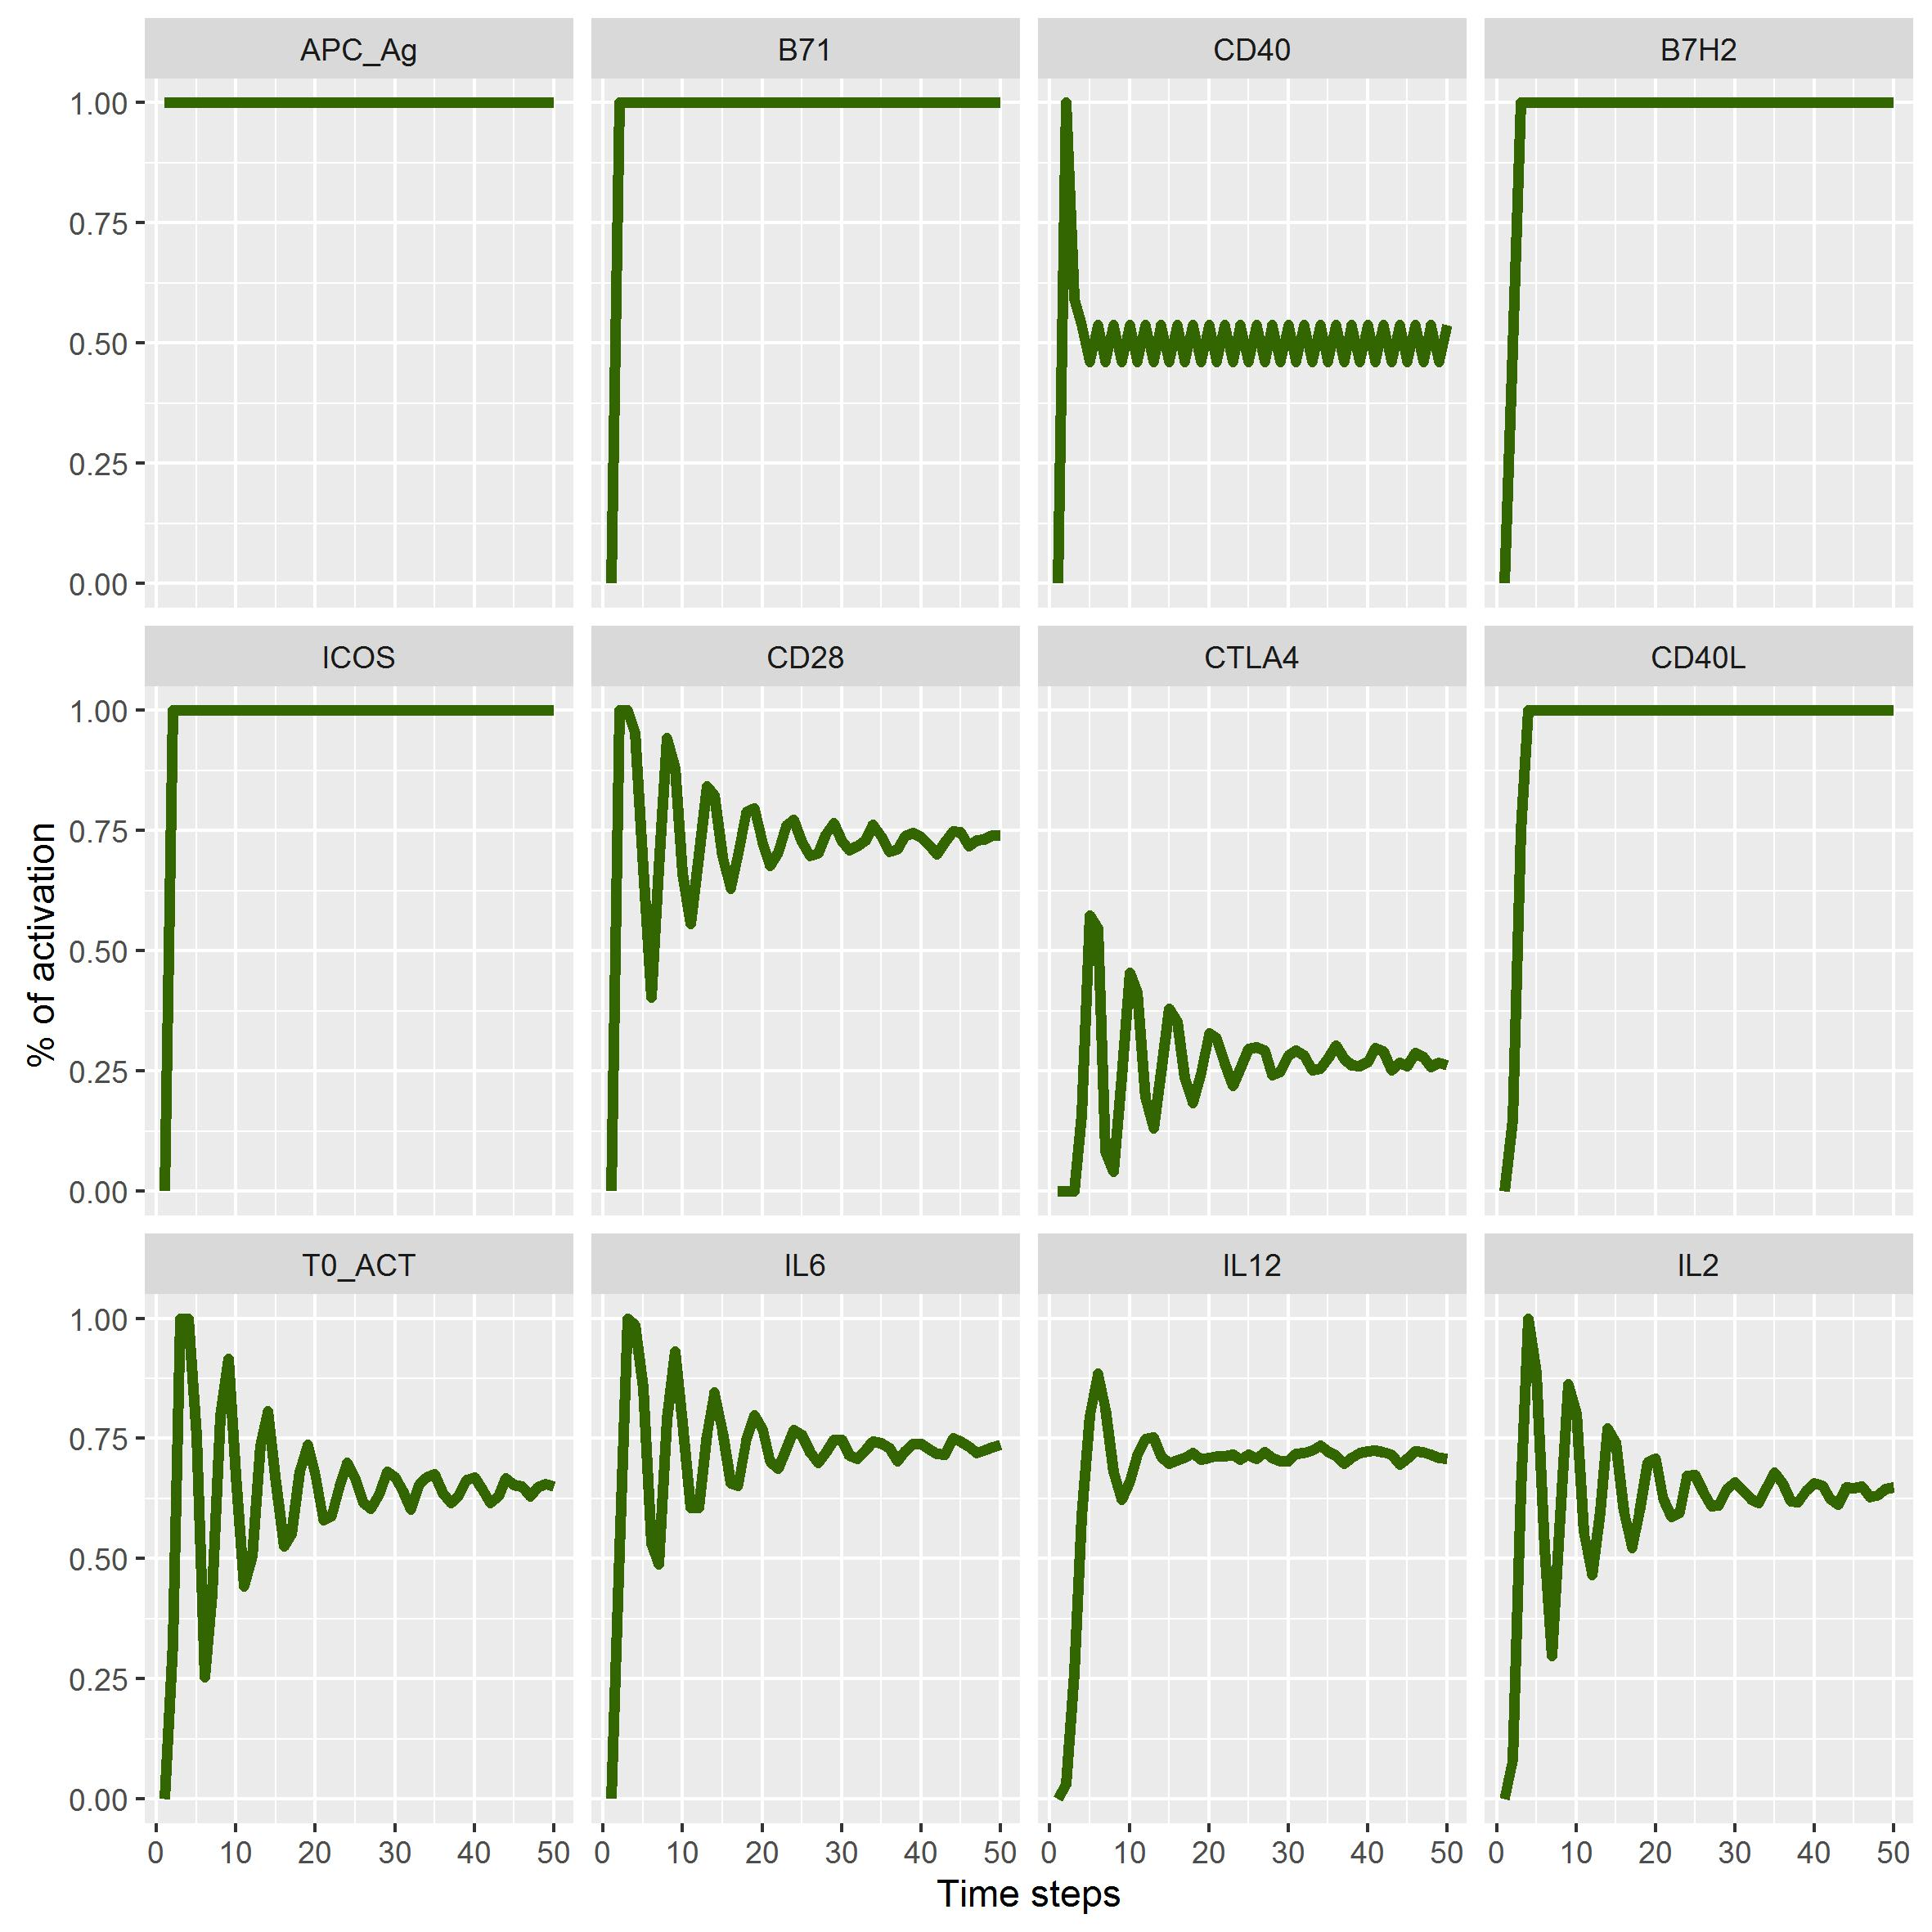
\includegraphics{Average.jpg}}
\caption{Average evolution of the network after 50 time steps in asynchronous mode.}\label{fig:Average}
\end{figure}

\subsection{Perturbation of the system}
In order to know which node perturbations can result in a significant change of the network dynamics, we can manipulate the system by knocking out or overexpressing the nodes. A knockout implies the deactivation of a component during all the simulation, whereas an overexpression generates a persistent activation of a node. Another possibility is to overexpress a node but only after its first activation or to activate/deactivate a node for some iterations. The majority of the function of SPIDDOR have arguments to introduce these perturbations:
\begin{itemize}
  \item{KO\_nodes:}{ A character vector with the name of the nodes to knockout (fixed to 0) over all the simulations(empty by default).}
  \item{Over\_expr:}{ A character vector with the name of the nodes to overexpress (fixed to 1) over all the simulations (empty by default).}
  \item{Over\_expr\_AA:}{ A character vector with the name of the nodes to overexpress (fixed to 1) after their first activation (empty by default).}
  \item{KO\_times:}{ A numeric vector specifying the iterations where the nodes in KO\_nodes argument will be fixed to 0. If empty the knockout is applied to the nodes for the entire simulation (empty by default).}
  \item{OE\_times:}{ A numeric vector specifying the iterations where the nodes in Over\_expr argument will be fixed to 1. If empty the overexpression is applied to the nodes for the entire simulation (empty by default).}
\end{itemize}

For example, to knock out ICOS when computing the dynamic evolution of the example network, we call:
\begin{Schunk}
\begin{Sinput}
> data(Example_network)
> BN <- read.Boolean.functions(Lines=BN$BooleanFunctions)
\end{Sinput}
\end{Schunk}
\texttt{\#Dynamic evolution of the network with a knockout in ICOS:}
\begin{Schunk}
\begin{Sinput}
> P_KOICOS<-dynamic_evolution.f(BN,time.steps=19,KO_nodes="ICOS",asynchronous = T)
> P_KOICOS["ICOS",]
\end{Sinput}
\end{Schunk}
\begin{verbatim}
 1  2  3  4  5  6  7  8  9 10 11 12 13 14 15 16 17 18 19 20 
 0  0  0  0  0  0  0  0  0  0  0  0  0  0  0  0  0  0  0  0 
\end{verbatim}
But if we only want to knock out ICOS from time step 5 to 10, we call:
\begin{Schunk}
\begin{Sinput}
> P_KOICOS2<-dynamic_evolution.f(BN,time.steps=19,KO_nodes="ICOS",
+                                KO_times=seq(5,10),asynchronous = T)
> P_KOICOS2["ICOS",]
\end{Sinput}
\end{Schunk}
\begin{verbatim}
 1  2  3  4  5  6  7  8  9 10 11 12 13 14 15 16 17 18 19 20 
 0  1  1  1  0  0  0  0  0  0  1  1  1  1  1  1  1  1  1  1 
\end{verbatim}

To knockout ICOS and B71, one from time step 5 to 10 and the other from time step 10 to 15:
\begin{Schunk}
\begin{Sinput}
> P_KOICOS_B71<-dynamic_evolution.f(BN,time.steps=19,KO_nodes=c("ICOS","B71"), 
+                                   KO_times=list(seq(5,10),seq(10,15)),
+                                   asynchronous = T)
> P_KOICOS_B71[c("ICOS","B71"),]
\end{Sinput}
\end{Schunk}
\begin{verbatim}
     1 2 3 4 5 6 7 8 9 10 11 12 13 14 15 16 17 18 19 20
ICOS 0 1 1 1 0 0 0 0 0  0  1  1  1  1  1  1  1  1  1  1
B71  0 1 1 1 1 1 1 1 1  0  0  0  0  0  0  1  1  1  1  1
\end{verbatim}

To overexpress node CD40L after its first activation when compunting the average trajectory of the network, we use: 
\begin{Schunk}
\begin{Sinput}
> AVG_OE_CD40L<-Average_simulations.f(BN,time.steps=19,Over_expr_AA = "CD40L",
+                                    asynchronous = TRUE,repetitions=2500)
> AVG_OE_CD40L["CD40L"]
\end{Sinput}
\end{Schunk}
\begin{verbatim}
    1     2     3     4     5     6     7     8     9    10    11    12 ...
0.000 0.159 0.755 1.000 1.000 1.000 1.000 1.000 1.000 1.000 1.000 1.000
\end{verbatim}


Additionally, users can change the activity level of the nodes in order to introduce ``polymorphisms-like'' mutations that, instead of completely deactivating a component of the network, they decrease the activity of a node to a lower extent (75\%, 50\%, 25\%...). This can be done easily by setting the ranges of the activity of the nodes in the \texttt{Polymorphism} argument from the \texttt{BN} class from 0 to 1 (0\% activity, 100\%activity). In the next example, we decrease the activity level of B71 node to 50\%.
\begin{Schunk}
\begin{Sinput}
> BN$Polymorphism["B71"]=0.5
> print(BN$Polymorphism)
\end{Sinput}
\end{Schunk}
\begin{verbatim}
APC_Ag    B71   CD40   B7H2   ICOS   CD28  CTLA4  CD40L T0_ACT    IL6   IL12    IL2 
   1.0    0.5    1.0    1.0    1.0    1.0    1.0    1.0    1.0    1.0    1.0    1.0 
\end{verbatim}
\begin{Schunk}
\begin{Sinput}
> AVG_B7150<-Average_simulations.f(BN,time.steps=19,Over_expr_AA = "CD40L",
+                                    asynchronous = TRUE,repetitions=5000)
> print(AVG_B7150["B71",])
\end{Sinput}
\end{Schunk}
\begin{verbatim}
    1     2     3     4     5     6     7     8     9    10    11    12 ...
0.000 0.501 0.493 0.502 0.509 0.494 0.489 0.495 0.499 0.505 0.506 0.501
\end{verbatim}

\section{Attractors}
Boolean models eventually evolve into a limited set of stable states known as attractors \cite{Hopfensitz2012-pv}. SPIDDOR is able to identify attractors using synchronous and asynchronous updating methods. An attractor can be a fixed-point if it consists on only one state, a simple cycle if it is composed by more than one state that oscillate in a cycle or a complex attractor if the set of states oscillate irregularly (due to the randomness involved in asynchronous networks). In our models the states of the nodes in the current iteration not only depend on the states of the nodes in the previous step, but also on prior steps due to the temporal predicates implemented with SPIDDOR. This produces an additional attractor type using the synchronous attractor search that we called ``complex cycle'', which consists on regular cycles with duplicated states.
\\
The \texttt{Get\_Attractor.f} function gets the attractor using the synchronous or asynchronous updating methods starting from an initial condition. To demonstrate this we will use the cell cycle Boolean network from \cite{Faure2006-ha}.

\begin{Schunk}
\begin{Sinput}
> data(cellcycle)
> print(BN_cellcycle)
\end{Sinput}
\end{Schunk}
\begin{verbatim}
$nodes.names
 [1] "CycD"   "Rb"     "E2F"    "CycE"   "CycA"   "p27"    "Cdc20"  "Cdh1"   "UbcH10"
[10] "CycB"  

$Initial_conditions
[1] "CycD"

$Modulator
named numeric(0)

$Arguments
numeric(0)

$Polymorphism
  CycD     Rb    E2F   CycE   CycA    p27  Cdc20   Cdh1 UbcH10   CycB 
     1      1      1      1      1      1      1      1      1      1 

$BooleanFunctions
 [1] "CycD= CycD"                                                                                    
 [2] "Rb= (! CycA & ! CycB & ! CycD & ! CycE) | (p27 & ! CycB & ! CycD)"                             
 [3] "E2F= (! Rb & ! CycA & ! CycB) | (p27 & ! Rb & ! CycB)"                                         
 [4] "CycE= (E2F & ! Rb)"                                                                            
 [5] "CycA= (E2F & ! Rb & ! Cdc20 & ! (Cdh1 & UbcH10)) | (CycA & ! Rb & ! Cdc20 
      & ! (Cdh1 & UbcH10))"
 [6] "p27= (! CycD & ! CycE & ! CycA & ! CycB) | (p27 & ! (CycE & CycA) 
      & ! CycB &! CycD)"           
 [7] "Cdc20= CycB"                                                                                   
 [8] "Cdh1=(! CycA & ! CycB) | (Cdc20) | (p27 & ! CycB)"                                             
 [9] "UbcH10= ! Cdh1 | (Cdh1 & UbcH10 & (Cdc20 | CycA | CycB))"                                      
[10] "CycB= ! Cdc20 & ! Cdh1"
\end{verbatim}

\texttt{\#Create the simulation algorithm for the cell cycle network}
\begin{Schunk}
\begin{Sinput}
> BN_cellcycle <- read.Boolean.functions(Lines=BN_cellcycle$BooleanFunctions)
\end{Sinput}
\end{Schunk}
\texttt{\#Get the attractor using the synchronous search (asynchronous=FALSE):}
\begin{Schunk}
\begin{Sinput}
> Attractor_syn<-Get_Attractor.f(BN_cellcycle,asynchronous=FALSE,Percent.ON=FALSE)
> print(Attractor_syn)
\end{Sinput}
\end{Schunk}
\begin{verbatim}
  CycD Rb E2F CycE CycA p27 Cdc20 Cdh1 UbcH10 CycB
1    1  0   1    0    0   0     0    1      1    0
2    1  0   1    1    0   0     0    1      0    0
3    1  0   1    1    1   0     0    1      0    0
4    1  0   0    1    1   0     0    0      0    0
5    1  0   0    0    1   0     0    0      1    1
6    1  0   0    0    1   0     1    0      1    1
7    1  0   0    0    0   0     1    1      1    0
\end{verbatim}
If Percent.ON=TRUE is selected, the function returns the attractor represented with the probability of activation of the nodes. If Percent.ON=FALSE is chosen, it returns all the states that form the attractor in a data.frame. For this example, we get a cycle composed of 7 states. If we want to see this in \%ON without recalling to the function with Percent.ON=TRUE, we can type:
\begin{Schunk}
\begin{Sinput}
> print(apply(Attractor_syn,2,sum)/dim(Attractor_syn)[1])
\end{Sinput}
\end{Schunk}

\begin{verbatim}
  CycD     Rb    E2F   CycE   CycA    p27  Cdc20   Cdh1 UbcH10   CycB 
 1.000  0.000  0.429  0.429  0.571  0.000  0.286  0.571  0.571  0.286 
\end{verbatim}

If the asynchronous attractor search is used, the function looks for the attractor by re-computing the simulation algorithm several times with a large number of iterations (more than 1000). Therefore, an additional argument \texttt{repetitions} is needed. Even when few repetitions are selected, the algorithm estimates a good approximation of the final attractor, that is why, we recommend first to try with a number smaller that 20 for this argument.
\begin{Schunk}
\begin{Sinput}
> Attractor_asyn<-Get_Attractor.f(BN_cellcycle,repetitions=12,asynchronous=TRUE)
> print(Attractor_asyn)
\end{Sinput}
\end{Schunk}
\begin{verbatim}
  CycD     Rb    E2F   CycE   CycA    p27  Cdc20   Cdh1 UbcH10   CycB 
 1.000  0.000  0.404  0.404  0.542  0.000  0.322  0.576  0.580  0.307 
\end{verbatim}
If you compare the synchronous and asynchronous attractors, you can appreciate that they are not completely the same. This is because, with the synchronous attractor search we get a simple cycle, whereas with the asynchrnous search the attractor is a complex cycle.\\
\\
In some cases there is not enough information to specify the initial condition of a system and sampling of a multitude of initial conditions is necessary. For those interested in this feature, SPIDDOR includes the \texttt{Get\_all\_attractors.f} function. Now, we will select the cardiac gene regulatory network from \cite{Herrmann2012-gm}.
\begin{Schunk}
\begin{Sinput}
> data(Cardiac_network)
> print(BN_Cardiacnetwork$nodes.names)
\end{Sinput}
\end{Schunk}
\begin{verbatim}
 [1] "Isl1"             "canWnt"           "exogen_BMP2_II"   "Bmp2"            
 [5] "exogen_canWnt_II" "Tbx1"             "Nkx2_5"           "Dkk1"            
 [9] "Mesp1"            "Fgf8"             "Tbx5"             "Foxc1_2"         
[13] "GATAs"            "exogen_CanWnt_I"  "exogen_BMP2_I" 
\end{verbatim}
\begin{Schunk}
\begin{Sinput}
> BN_Cardiacnetwork<-read.Boolean.functions(Lines=BN_Cardiacnetwork$BooleanFunctions)
\end{Sinput}
\end{Schunk}
This network has 15 nodes, so the possible initial conditions to test are 32768 ($2^{15}$). As the number of initial conditions to test grow exponentially with the number of nodes, \texttt{Get\_all\_attractors.f} function searches all the attractors for networks with less than 20 nodes. For larger networks, we allow the specification of a subset of nodes (<20) in \texttt{BN\$Initial\_conditions} in which all the combination of nodes will be tested, or the specification of a number of starting states to test (<100,000). Furthermore, this algorithm is parallelized using the snowfall library \cite{Knaus2013-py}, so the user must specified the number of cpus to use. In the next example, we use 4 cpus and the synchronous search to get all the attractors of the cardiac network:

\begin{Schunk}
\begin{Sinput}
> All_attr_syn<-Get_all_attractors.f(cpus=4,BN_Cardiacnetwork,asynchronous=FALSE)
> print(All_attr_syn)
\end{Sinput}
\end{Schunk}
\begin{verbatim}
  Isl1 canWnt exogen_BMP2_II Bmp2 exogen_canWnt_II Tbx1 Nkx2_5 Dkk1 Mesp1 Fgf8 Tbx5
1    0      0              1    1                0    0      0    0     0    0    0
2    0      0              1    1                0    0      1    0     0    0    1
3    1      1              1    0                1    1      1    0     0    1    0
  Foxc1_2 GATAs exogen_CanWnt_I exogen_BMP2_I  Recurrence
1       0     0               0             1 0.007263184
2       0     1               0             1 0.492736816
3       1     1               1             1 0.500000000
\end{verbatim}

If we want to get the attractors by only checking 1000 random initial states, we call:

\begin{Schunk}
\begin{Sinput}
> All_attr_syn<-Get_all_attractors.f(cpus=4,BN_Cardiacnetwork,asynchronous=FALSE,
+                                    startStates=1000)
> print(All_attr_syn)
\end{Sinput}
\end{Schunk}
\begin{verbatim}
  Isl1 canWnt exogen_BMP2_II Bmp2 exogen_canWnt_II Tbx1 Nkx2_5 Dkk1 Mesp1 Fgf8 Tbx5
1    0      0              1    1                0    0      0    0     0    0    0
2    0      0              1    1                0    0      1    0     0    0    1
  Foxc1_2 GATAs exogen_CanWnt_I exogen_BMP2_I Recurrence
1       0     0               0             1       0.06
2       0     1               0             1       0.94
\end{verbatim}

By only checking 1000 initial states we do not get the third fixed-point of the network.
\section{Perturbation analysis}
\texttt{KO\_matrix.f} function evaluates the effect of single node knockouts on the network by computing the Perturbation index ($Prob_{Perturbed} / Prob_{Normal}$) of the nodes. The result of this function is a square matrix indicating how the knockout of the ``column node'' affects each ``row node''.\\
\texttt{OE\_matrix.f} function is equal to the previous function but it evaluates the effects of ``overexpressions after activation'' on the nodes of the network.

\texttt{Create\_heatmap} function is used to visualize the individual values contained in the matrix returned by these two functions as colors with a heatmap of the column nodes. The perturbations that lead to a higher activation of the nodes compared to an unperturbed situation are represented in orange while a lower activation of the nodes is indicated in blue. This color palette can be changed by the user.


\begin{Schunk}
\begin{Sinput}
> data(Example_network)
> BN <- read.Boolean.functions(Lines=BN$BooleanFunctions)
> KO.m<-KO_matrix.f(BN,time_steps=999,repetitions=24,asynchronous=TRUE)
> Create_heatmap(KO.m)
\end{Sinput}
\end{Schunk}
\begin{figure}[!htbp]
\centerline{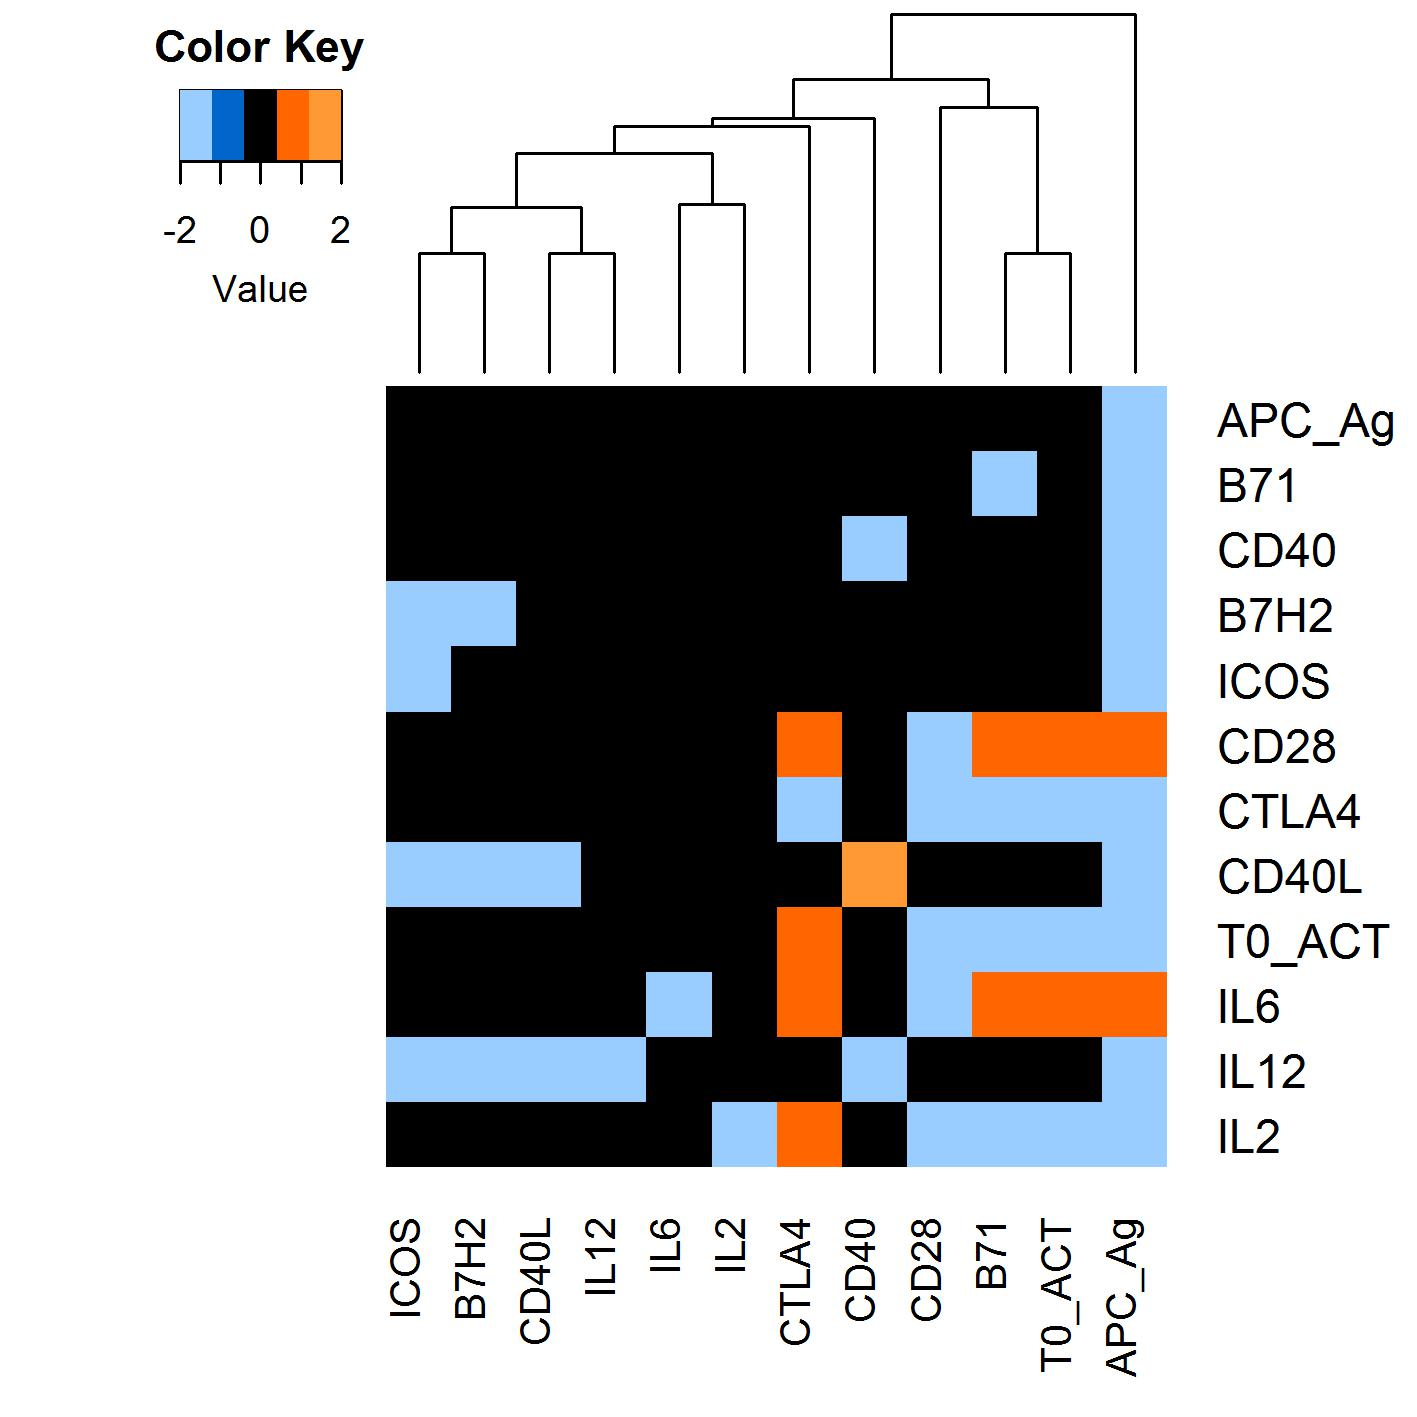
\includegraphics{heatmap.jpg}}
\end{figure}


\section{Model interoperability}
The \texttt{export2SBMLqual} function is used to convert the BFs of the user's text file to the SBML qual format\cite{Chaouiya2013-ov}. The output file is saved in .sbml extension, and can be imported to other Boolean analysis tools like GINsim\cite{Gonzalez2006-up} or BoolNet\cite{Mussel2010-zu} (both platforms are part of the CoLoMoTo Consortium \cite{Naldi2015-jp}).

\begin{Schunk}
\begin{Sinput}
> data(Cardiac_network)
> export2SBMLqual(Lines=BN_Cardiacnetwork$BooleanFunctions,file="cardiac_network.sbml")
\end{Sinput}
\end{Schunk}

\clearpage

\bibliographystyle{plain}
\bibliography{SPIDDOR_bib}

\end{document}
